% !TEX program = xelatex
% !TEX TS-program = xelatex
% !TEX encoding = UTF-8
% ↑ LaTeX Workshop / latexmk 看到這行就會自動切到 xelatex（本檔案用 fontspec + xeCJK，pdflatex 跑不動）

\documentclass[11pt,a4paper]{article}

% ─── 引擎與中文 ─────────────────────────────────────
\usepackage{fontspec}
\usepackage{xeCJK}
\usepackage{amsmath}
\setCJKmainfont[
  BoldFont={Source Han Serif TW Bold},
  ItalicFont={Source Han Serif TW Light},
]{Source Han Serif TW}
\setCJKsansfont{Source Han Serif TW Medium}
\setCJKmonofont{Source Han Serif TW}
\setmainfont{Latin Modern Roman}
\setmonofont[Scale=0.9]{Latin Modern Mono}
\xeCJKsetup{CJKecglue={\hskip 0.15em plus 0.05em minus 0.05em}}

% ─── 排版 ───────────────────────────────────────────
\usepackage[a4paper,top=2.2cm,bottom=2.2cm,left=2.3cm,right=2.3cm]{geometry}
\usepackage{graphicx}
\usepackage{xcolor}
\usepackage{hyperref}
\usepackage{enumitem}
\usepackage{titlesec}
\usepackage{fancyhdr}
\usepackage{tabularx}
\usepackage{booktabs}
\usepackage{tikz}
\usepackage{caption}
\usepackage{float}
\usepackage{placeins} % \FloatBarrier
\usepackage{multicol}
\usetikzlibrary{positioning,shapes.geometric,arrows.meta,fit,backgrounds,calc}

% 行距舒適
\linespread{1.18}

% ─── 顏色 ───────────────────────────────────────────
\definecolor{brand}{HTML}{0EA5E9}
\definecolor{brandDeep}{HTML}{0369A1}
\definecolor{ink}{HTML}{0F172A}
\definecolor{mute}{HTML}{64748B}
\definecolor{paper}{HTML}{F8FAFC}
\definecolor{accent}{HTML}{10B981}
\definecolor{warn}{HTML}{F59E0B}
\definecolor{danger}{HTML}{EF4444}

\hypersetup{
  colorlinks=true,
  linkcolor=brandDeep,
  urlcolor=brandDeep,
  citecolor=brandDeep,
  pdftitle={台大水資源問題地圖｜期末書面報告},
  pdfauthor={NTU Water Risk Map},
  plainpages=false,
}

% ─── 標題 ───────────────────────────────────────────
\titleformat{\section}
  {\Large\bfseries\color{brandDeep}}
  {\thesection.}{0.6em}{}[\vspace{-0.2em}\color{brand}\rule{\linewidth}{0.6pt}]
\titleformat{\subsection}
  {\large\bfseries\color{ink}}
  {\thesubsection}{0.6em}{}
\titlespacing*{\section}{0pt}{1.4em}{0.6em}
\titlespacing*{\subsection}{0pt}{1.0em}{0.4em}

% ─── 頁首頁尾 ───────────────────────────────────────
\setlength{\headheight}{14pt}
\pagestyle{fancy}
\fancyhf{}
\fancyhead[L]{\small\color{mute}台大水資源問題地圖｜期末報告}
\fancyhead[R]{\small\color{mute}NTU Water Risk Map}
\fancyfoot[C]{\small\color{mute}\thepage}
\renewcommand{\headrulewidth}{0.3pt}
\renewcommand{\footrulewidth}{0pt}

\captionsetup{font=small,labelfont={bf,color=brandDeep},labelsep=quad,skip=6pt}

% ─── 自訂 box ───────────────────────────────────────
\usepackage[breakable,skins]{tcolorbox}
\newtcolorbox{infobox}[1][]{
  enhanced, colback=paper, colframe=brand!40, arc=2mm, boxrule=0.5pt,
  left=10pt,right=10pt,top=7pt,bottom=7pt, breakable, fontupper=\small, #1
}
\newtcolorbox{techbox}[1][]{
  enhanced, colback=brandDeep!4, colframe=brandDeep!50, arc=2mm, boxrule=0.5pt,
  left=10pt,right=10pt,top=7pt,bottom=7pt, breakable, fontupper=\small, #1
}
\newtcolorbox{warnbox}[1][]{
  enhanced, colback=warn!8, colframe=warn!50, arc=2mm, boxrule=0.5pt,
  left=10pt,right=10pt,top=7pt,bottom=7pt, breakable, fontupper=\small, #1
}
\newtcolorbox{accentbox}[1][]{
  enhanced, colback=accent!8, colframe=accent!50, arc=2mm, boxrule=0.5pt,
  left=10pt,right=10pt,top=7pt,bottom=7pt, breakable, fontupper=\small, #1
}

\setlist[itemize]{leftmargin=1.4em,topsep=2pt,itemsep=2pt,parsep=0pt}
\setlist[enumerate]{leftmargin=1.6em,topsep=2pt,itemsep=2pt,parsep=0pt}

% 圖表浮動參數：盡量讓 figure 留在原位
\setcounter{topnumber}{2}
\setcounter{bottomnumber}{2}
\setcounter{totalnumber}{4}
\renewcommand{\topfraction}{0.95}
\renewcommand{\bottomfraction}{0.95}
\renewcommand{\textfraction}{0.05}
\renewcommand{\floatpagefraction}{0.85}

% 截圖統一寬度，整齊一致
\newcommand{\screenfig}[3]{%
  \begin{figure}[H]\centering
    \includegraphics[width=#1\linewidth,#2]{screens/#3}%
  \end{figure}%
}

\begin{document}

% ═══════════════════════════════════════════════════════
% P.1 — 封面
% ═══════════════════════════════════════════════════════
\begin{titlepage}
\thispagestyle{empty}
\centering
\vspace*{1.2cm}

\begin{tikzpicture}
\node[circle,fill=brand,minimum size=2.6cm] (logo) {};
\node at (logo) {\color{white}\fontsize{36}{36}\selectfont \textbf{水}};
\end{tikzpicture}

\vspace{1.0cm}
{\color{mute}\large NTU Water Resource Project~~$\bullet$~~Final Report}\\[0.4cm]

{\color{ink}\fontsize{32}{38}\selectfont\bfseries 台大水資源問題地圖}\\[0.5cm]
{\color{brandDeep}\Large NTU Water Risk Map}\\[0.6cm]
{\color{mute}\large 校園即時回報、雨天導航、水災預警一站式平台}\\[2.2cm]

\begin{tcolorbox}[
  enhanced, colback=paper, colframe=brand!30,
  arc=3mm, boxrule=0.6pt, width=0.82\linewidth,
  left=20pt,right=20pt,top=16pt,bottom=16pt,
]
\renewcommand{\arraystretch}{1.6}
\begin{tabularx}{\linewidth}{@{}lX@{}}
\textbf{\color{brandDeep}課程} & 水資源工程與管理（期末專題）\\
\textbf{\color{brandDeep}類型} & Web Application — 互動式校園地圖平台\\
\textbf{\color{brandDeep}技術棧} & Next.js 14 / TypeScript / React Leaflet / Recharts \\
\textbf{\color{brandDeep}資料源} & OpenStreetMap、中央氣象署、台北自來水處 OpenData\\
\textbf{\color{brandDeep}部署} & Vercel（hnd1 / 東京區域，10 個 API Routes）\\
\textbf{\color{brandDeep}日期} & 2026 年 5 月 \\
\end{tabularx}
\end{tcolorbox}

\vfill


\begin{tikzpicture}
\foreach \x/\c in {0/brand, 0.8/brandDeep, 1.6/accent, 2.4/warn, 3.2/danger}
  \node[circle,fill=\c,minimum size=0.42cm] at (\x,0) {};
\end{tikzpicture}

\vspace{0.3cm}
{\color{mute}\small \textit{Make rainy-day campus walking less wet, one node at a time.}}
\vspace{0.5cm}
\end{titlepage}

% ═══════════════════════════════════════════════════════
% P.2 — 摘要 + 動機
% ═══════════════════════════════════════════════════════
\section{摘要}

本專題以「水資源問題」為核心，為台大師生開發一套\textbf{校園即時水情平台} —— 結合
\emph{眾包回報}、\emph{即時氣象}、\emph{校園路網最佳化}與\emph{數據儀表板}，把分散在校園各角落的積水、漏水、淹水資訊集中視覺化，並進一步轉化為「下一步該怎麼走、該怎麼避」的具體建議。

不同於傳統紙本問卷或單向公告，本平台採取\textbf{雙向數據迴圈}：使用者回報的問題會即時影響其他人的雨天路徑規劃；\emph{校方管理端}可從儀表板與 CSV 匯出觀察高風險點，作為改善決策依據。
全站共 6 個主要頁面、10 個 Node.js API Routes，整合 3 項外部資料源，路徑規劃部分以 Dijkstra（雙層 GeoJSON 路網，6{,}133 節點、7{,}248 條邊）即時計算最低淋雨成本。

\begin{infobox}
\textbf{\color{brandDeep}核心成果一覽}
\begin{itemize}
\item \textbf{6 頁面}：地圖首頁、雨天路徑、水災預警、儀表板、個人成績單、管理後台
\item \textbf{4 大問題類別}：淹水 / 積水 / 設施漏水 / 排水不良；3 級嚴重度與 4 種處理狀態
\item \textbf{路徑演算法}：以 OSM tags 推論遮蔽率（\texttt{indoor/tunnel/covered/arcade}），雨大時可在僅多走 $\sim$50 m 的條件下將遮蔽率提升 30\,\%+
\item \textbf{眾包飲水機地圖}：融合 OSM 社群 + 北水處官方 OpenData，26 台校內飲水機可即時報修、+1 減塑
\item \textbf{減塑量化}：每 +1 換算為一個 600 mL 寶特瓶與 14 g CO\textsubscript{2}\,e 節省量
\end{itemize}
\end{infobox}

\section{動機與問題定義}

\textbf{校園裡有水的問題嗎？有，而且很多。} 椰林大道兩側下大雨會嚴重積水、總圖前廣場常有低窪滯水、活大附近設施漏水、某些飲水機壞了沒人通報、學生不知道哪條路最少淋雨 —— 這些都是真實但「\emph{知道的人很零散}」的問題。

我們的觀察：\emph{資訊在校園裡是孤島}。校方有官方申報系統但回報門檻高；學生在 Threads / Dcard 抱怨但訊息無法被追蹤；氣象署的雨量資料與校園座標毫無關聯。本專題希望以一個輕量、即時、地圖中心的 web app，把「\textbf{回報} → \textbf{視覺化} → \textbf{行為改變}」串成閉環。

\begin{warnbox}
\textbf{\color{warn!70!black}三個底層問題與解法}
\begin{enumerate}
\item \textbf{回報沒人理}：傳統表單填了之後不知道有沒有人看 $\Rightarrow$ 用\emph{眾包確認機制（still\_exists / resolved）}讓社群相互驗證。
\item \textbf{雨天還是用 Google Maps}：但 GMaps 不知道椰林大道哪段有騎樓 $\Rightarrow$ 用\emph{OSM 抓的密集路網} + \emph{雨勢加權 Dijkstra} 給出真正避雨的走法。
\item \textbf{看數據的人不在地圖前}：校方需要的是趨勢與排行 $\Rightarrow$ 用\emph{14 天趨勢 + 風險分數排行 + 處理 SLA} 的儀表板。
\end{enumerate}
\end{warnbox}

\clearpage

% ═══════════════════════════════════════════════════════
% P.3 — 系統架構（圖獨立成頁開頭）
% ═══════════════════════════════════════════════════════
\section{系統架構}

採用 Next.js 14 App Router 的 \textbf{Server Components + 邊緣化 API} 架構：
圖資與演算法重的工作（3 MB GeoJSON 載入、Dijkstra 計算、CWA API 代理）放在 server-side；地圖互動與 UI 在 client。整體分為五層：\textbf{Client 頁面} $\to$ \textbf{API Routes} $\to$ \textbf{演算法層} $\to$ \textbf{內部資料} $\to$ \textbf{外部公開資料源}。

\begin{figure}[H]
\centering
\begin{tikzpicture}[
  every node/.style={font=\scriptsize, transform shape},
  box/.style={
    rectangle, rounded corners=2.5pt, draw=brand!50, fill=white,
    minimum height=0.62cm, inner xsep=4pt, inner ysep=3pt, align=center,
  },
  client/.style={box, fill=brand!12,    draw=brand!70,     minimum width=2.18cm, minimum height=0.95cm},
  api/.style   ={box, fill=brandDeep!8, draw=brandDeep!70, minimum width=15.6cm, minimum height=1.05cm},
  algo/.style  ={box, fill=accent!12,   draw=accent!70,    minimum width=15.6cm, minimum height=0.75cm},
  data/.style  ={box, fill=accent!8,    draw=accent!60,    minimum width=4.9cm,  minimum height=1.05cm},
  ext/.style   ={box, fill=warn!12,     draw=warn!60,      minimum width=4.9cm,  minimum height=1.05cm},
  arr/.style   ={-Stealth, line width=0.6pt, brandDeep!75, shorten >=2pt, shorten <=2pt},
  arrext/.style={-Stealth, line width=0.6pt, warn!70!black!85, shorten >=2pt, shorten <=2pt, dashed},
  lane/.style  ={rectangle, rounded corners=2pt, fill=#1, draw=none},
  lanetag/.style={font=\footnotesize\bfseries, color=#1, anchor=west, inner sep=2pt, align=left, text width=1.6cm},
]

% ── Layer Y-coordinates (wider gaps to avoid arrow overlap with boxes) ──
\def\yClient{9.6}
\def\yApi{7.7}
\def\yLogic{6.1}
\def\yData{4.4}
\def\ySource{2.6}

% ── Swim-lane backgrounds (subtle, full-width) ──
\begin{scope}[on background layer]
  \fill[brand!4]    (-0.3, \yClient-0.7) rectangle (16.6, \yClient+0.7);
  \fill[brandDeep!3](-0.3, \yApi   -0.7) rectangle (16.6, \yApi   +0.7);
  \fill[accent!4]   (-0.3, \yLogic -0.5) rectangle (16.6, \yLogic +0.5);
  \fill[accent!3]   (-0.3, \yData  -0.7) rectangle (16.6, \yData  +0.7);
  \fill[warn!4]     (-0.3, \ySource-0.7) rectangle (16.6, \ySource+0.7);
\end{scope}

% ── Lane tags (right-side, vertical-centered with each band) ──
\node[lanetag=brand!70!black]    at (16.7, \yClient) {Client \\ \scriptsize\color{mute}\textmd{6 個頁面}};
\node[lanetag=brandDeep!70]      at (16.7, \yApi)    {API \\ \scriptsize\color{mute}\textmd{10 endpoints}};
\node[lanetag=accent!50!black]   at (16.7, \yLogic)  {Logic \\ \scriptsize\color{mute}\textmd{演算法}};
\node[lanetag=accent!50!black]   at (16.7, \yData)   {Data \\ \scriptsize\color{mute}\textmd{內部儲存}};
\node[lanetag=warn!60!black]     at (16.7, \ySource) {Source \\ \scriptsize\color{mute}\textmd{外部 API}};

% ── Layer 1: Client (6 pages) ──
\node[client]                            (home)     at (1.2, \yClient) {\textbf{/}\\首頁地圖};
\node[client, right=0.30cm of home]      (route)                       {\textbf{/route}\\雨天路徑};
\node[client, right=0.30cm of route]     (forecast)                    {\textbf{/forecast}\\水災預警};
\node[client, right=0.30cm of forecast]  (dash)                        {\textbf{/dashboard}\\儀表板};
\node[client, right=0.30cm of dash]      (me)                          {\textbf{/me}\\個人成績};
\node[client, right=0.30cm of me]        (admin)                       {\textbf{/admin}\\管理後台};

% ── Layer 2: API Routes ──
\node[api] (apibox) at (7.95, \yApi) {%
  \textbf{Next.js API Routes}（10 endpoints, server-side）\\[1pt]
  \texttt{/api/\{reports, route, forecast, weather, stats, water-stations, path-geometry\}}
};

% ── Layer 3: Algorithm ──
\node[algo] (algobox) at (7.95, \yLogic) {%
  \textbf{演算法層}\;\;Dijkstra (denseGraph) $\cdot$ Risk Score $\cdot$ 90 天熱力預測 $\cdot$ Mock/Real 切換
};

% ── Layer 4: Internal Data ──
\node[data] (geo)   at ( 2.9, \yData) {\textbf{GeoJSON 路網}\\\scriptsize 6{,}133 nodes / 7{,}248 edges $\cdot$ server-only};
\node[data] (store) at ( 7.95, \yData) {\textbf{Mock / Supabase}\\\scriptsize reports + confirmations + storage};
\node[data] (local) at (13.0, \yData) {\textbf{LocalStorage}\\\scriptsize streak / badges / preferences (client)};

% ── Layer 5: External APIs ──
\node[ext] (osm) at ( 2.9, \ySource) {\textbf{OpenStreetMap}\\\scriptsize Overpass API $\cdot$ 校園路網與飲水機點位};
\node[ext] (twd) at ( 7.95, \ySource) {\textbf{臺北自來水處 OpenData}\\\scriptsize 飲水機水質 + 官方狀態};
\node[ext] (cwa) at (13.0, \ySource) {\textbf{中央氣象署 OpenData}\\\scriptsize O-A0003-001 / F-D0047-061};

% ── Arrows: 5 client pages → API ──
\foreach \src in {home, route, forecast, dash, admin} {
  \draw[arr] (\src.south) -- (\src.south |- apibox.north);
}
% me → 直連 LocalStorage（橫向斜線，繞過 API/Logic/Data 三層）
\draw[arr] (me.south) -- ++(0, -0.4)
  -| ($(local.north) + (0.6, 0.4)$) -- ($(local.north) + (0.6, 0)$);

% API → Algo
\draw[arr] (apibox.south) -- (algobox.north);

% Algo → 3 個 Internal data 框（從 algo 底邊三個垂直點下來）
\draw[arr] (algobox.south -| geo.north)   -- (geo.north);
\draw[arr] (algobox.south -| store.north) -- (store.north);
\draw[arr] (algobox.south -| local.north) -- (local.north);

% Internal data → External APIs (虛線：build-time / runtime fetch)
\draw[arrext] (geo.south)   -- (osm.north);
\draw[arrext] (store.south) -- (twd.north);
% CWA 來自 algo 直接 fetch（不經 internal store）— 從 algobox 右側繞下來
\draw[arrext] (algobox.east) -- ++(0.4, 0) |- (cwa.east);

% ── Legend (bottom-left, inside frame) ──
\node[anchor=west, font=\scriptsize, color=mute, inner sep=3pt]
  at (0, 1.1)
  {\tikz{\draw[arr] (0,0) -- (0.55,0);}\;\;內部呼叫 / 函式 \qquad
   \tikz{\draw[arrext] (0,0) -- (0.55,0);}\;\;外部 API（透過 server proxy）};

\end{tikzpicture}
\caption{系統五層架構（Swim-lane 視覺化）：Client 6 個頁面 → API Routes 10 endpoints → 演算法層 → 內部資料（GeoJSON / Mock / LocalStorage）→ 外部資料源（OSM / 北水處 / CWA）。實線=內部呼叫，虛線=外部 API。\texttt{/me} 直連 LocalStorage 不經 server 以保護隱私。}
\end{figure}

\clearpage

\subsection{技術選型理由}

\begin{techbox}
\renewcommand{\arraystretch}{1.25}
\begin{tabularx}{\linewidth}{@{}p{2.8cm}X@{}}
\textbf{Next.js 14} & App Router 提供 server-only 模組能力，3 MB 校園路網檔（\texttt{campus-paths.geojson}）只在 server 載入，client bundle 不受影響。\\
\textbf{React Leaflet} & 開源、無 API key 限制，可疊加自訂 GeoJSON 與多型 marker；用 \texttt{dynamic(\{ssr:false\})} 避開 SSR 的 \texttt{window} 問題。\\
\textbf{Recharts} & 比 Chart.js 更貼合 React 心智模型，原生支援響應式容器，方便嵌入 dashboard 卡片。\\
\textbf{Supabase（可選）} & 預設 \texttt{NEXT\_PUBLIC\_USE\_MOCK=true}，零配置可 demo；接上即得 PostgreSQL + Storage + RLS。\\
\textbf{Vercel hnd1} & 東京區域離台灣 RTT 最低，配合 \texttt{maxDuration:30s} 容許演算法 routes 載入大 GeoJSON。\\
\end{tabularx}
\end{techbox}

\subsection{資料流關鍵設計}

\begin{itemize}
\item \textbf{Mock 與真實環境同介面}：\texttt{lib/supabase.ts} 透過環境變數切換，前端程式碼完全不變 —— demo 時零配置，正式上線時切 Supabase。
\item \textbf{Server-side Heavy Compute}：Dijkstra 與 90 天熱力預測都在 \texttt{/api/route} 與 \texttt{/api/forecast} 計算，client 只收到 polyline 與機率格網，避免 3 MB 路網檔下載到瀏覽器。
\item \textbf{個人資料純本機}：\texttt{/me} 的連續打卡、徽章、行動分數都用 LocalStorage，零追蹤、隱私第一。
\end{itemize}

\clearpage

% ═══════════════════════════════════════════════════════
% 4. 核心功能展示
% ═══════════════════════════════════════════════════════
\section{核心功能展示 \quad \normalfont\normalsize\color{mute}— 5 個面向使用者的頁面，每節含實際畫面}

\subsection{地圖首頁 \texttt{/} — 一張地圖看完校園水情}

首頁採\textbf{地圖中心}（map-centric）設計：左側是互動式校園地圖，右側為四張資訊卡片（今日通勤、附近飲水機、高風險地點排行、最新回報）。使用者落地的 3 秒內可看到：(1) 校園有多少筆待處理問題、(2) 自己附近的飲水機狀態、(3) 該不該改走另一條路。

\begin{figure}[H]\centering
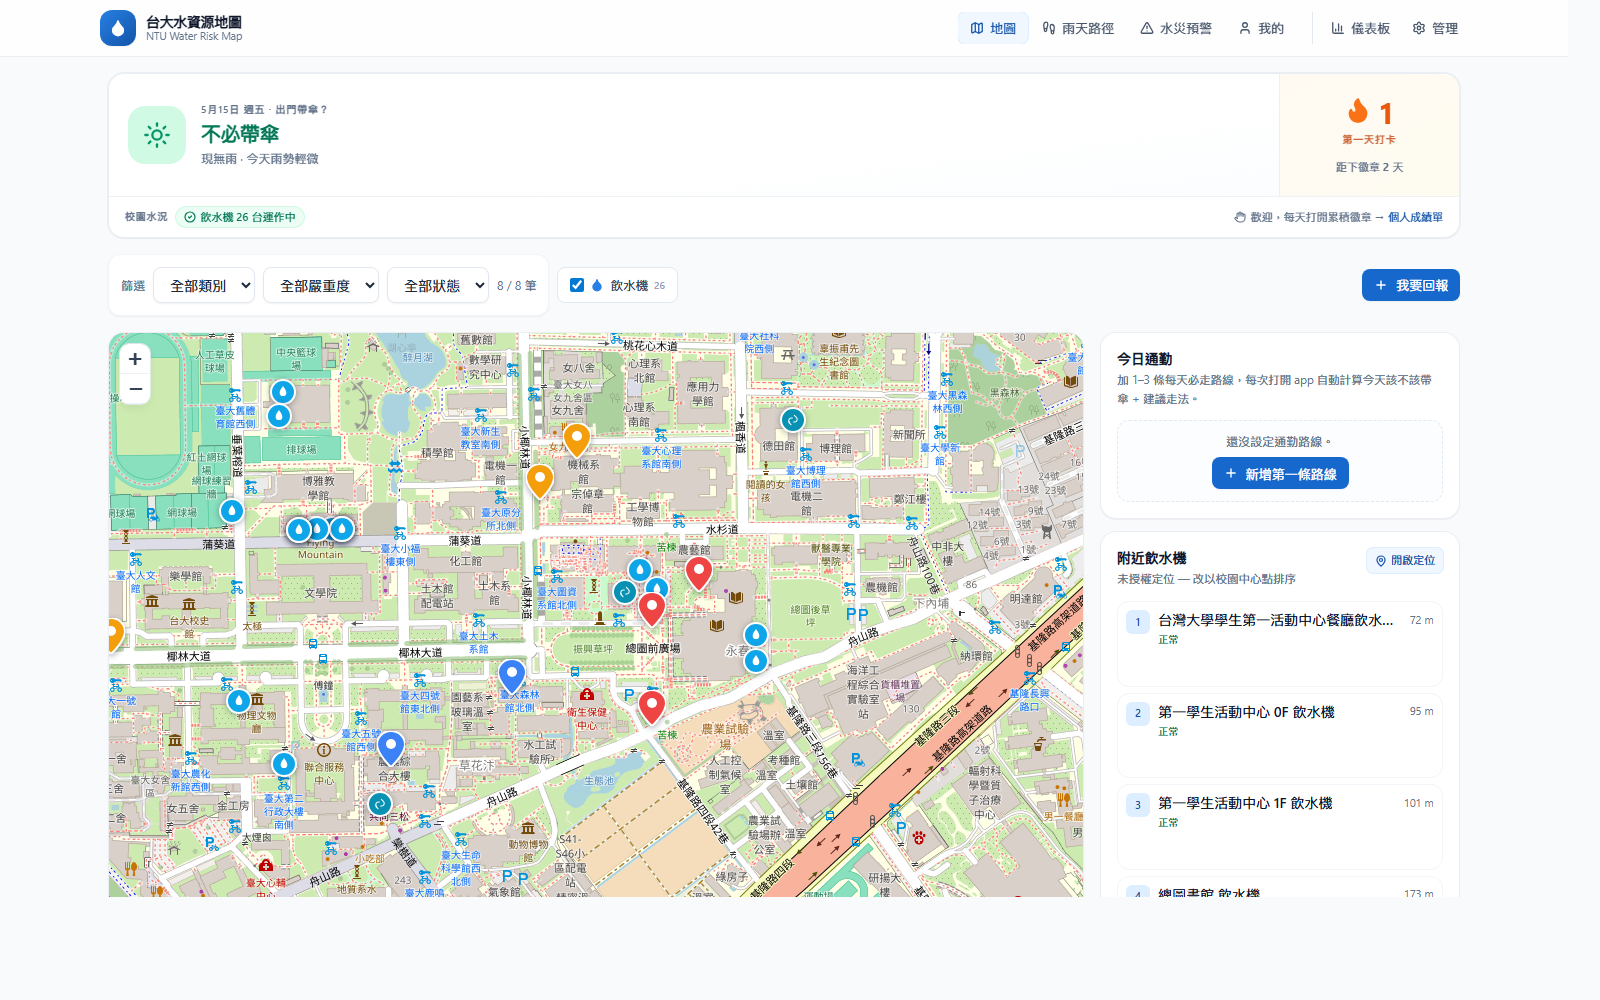
\includegraphics[width=0.96\linewidth]{screens/home.png}
\caption{首頁實際畫面：地圖以台大校園為中心顯示水資源回報（紅／橙／藍 = 嚴重度）與飲水機點位（藍水滴），右側為高風險地點排行（依 \texttt{risk\_score} 排序）。}
\end{figure}

\begin{infobox}
\textbf{\color{brandDeep}首頁亮點功能}
\begin{itemize}
\item \textbf{今日水情報（Today Briefing）}：根據即時氣象在頁面頂端動態生成「不必擔心」「準備雨具」「強烈建議帶傘」等口語化提示。
\item \textbf{雙層 markers 圖層切換}：可獨立顯示／隱藏 26 台飲水機與校園水資源回報，避免視覺擁擠。
\item \textbf{高風險地點排行（Risk Ranking）}：依分組座標計算 \texttt{risk\_score = reports$\times$2 + high$\times$3 + recent7d$\times$2}，點擊即跳到地圖該位置。
\item \textbf{回報眾包確認}：每筆 report 支援「\emph{還在}」「\emph{已解決}」雙向投票，自動更新 \texttt{upvote\_count} / \texttt{resolved\_count}。
\end{itemize}
\end{infobox}

\clearpage

\subsection{雨天路徑規劃 \texttt{/route} — 真實 OSM 路網 + 加權 Dijkstra}

關鍵差異化：\textbf{不是把 Leaflet polyline 畫一畫}，而是用\emph{加權 Dijkstra} 在真實 OSM 路網上做計算。地圖同時顯示\textbf{防雨建議路徑}（綠粗線）與\textbf{最短路徑}（灰虛線）作為對比，左側面板提供交通工具切換、雨勢 mock 滑桿、積水疊圖開關，並即時顯示\emph{遮蔽率提升}、\emph{易積水比例下降}、\emph{避開回報數}。

\begin{figure}[H]\centering
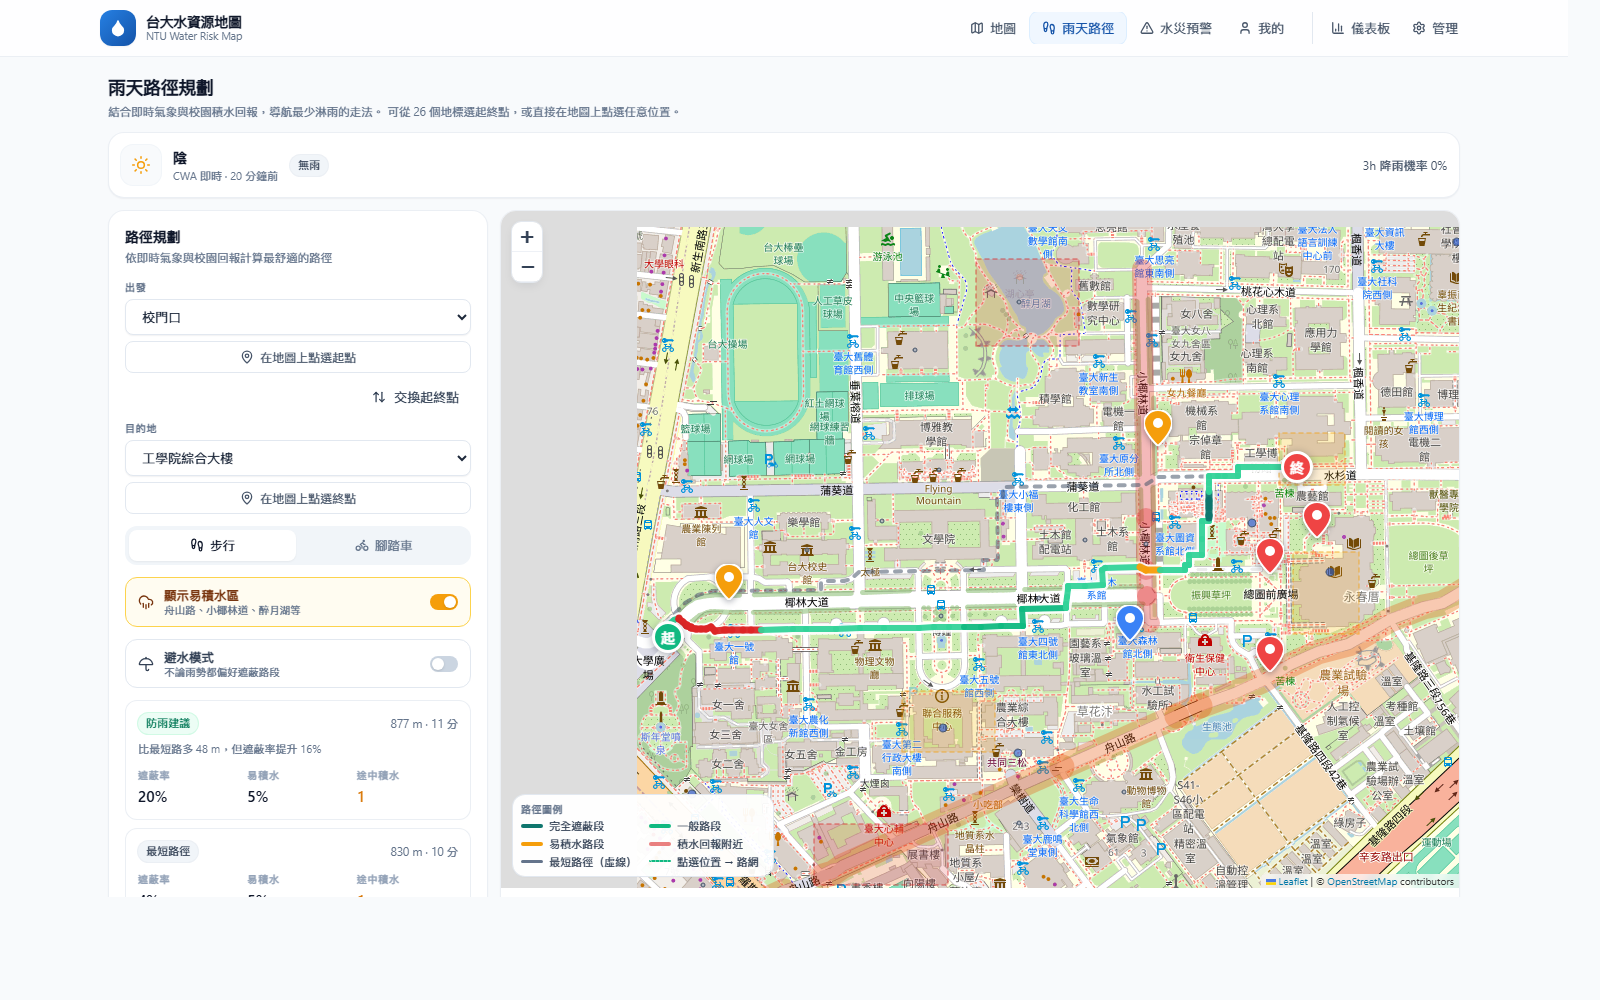
\includegraphics[width=0.96\linewidth]{screens/route.png}
\caption{雨天路徑規劃畫面：綠粗線為防雨建議路徑，灰虛線為最短路徑對照。地圖支援「點任一處設為起終點」，server 會 snap 到最近的 OSM 路網節點。}
\end{figure}

\textbf{邊權公式}（\texttt{src/lib/denseGraph.ts}）：
\[
\mathrm{cost} = d \times \bigl( 1 + r \times \bigl( 2.4(1{-}c) + 2.2\,\ell + 0.8\,f \bigr) \bigr)
\]

其中 $d$ = 距離、$r$ = 雨勢係數（CWA 即時雨量推算）、$c$ = 遮蔽率、$\ell$ = 是否低窪、$f$ = 該段附近積水回報數。雨大時 $r$ 變大，演算法會願意繞遠走有騎樓 / 室內走廊（\texttt{indoor=yes}、\texttt{arcade=yes}、\texttt{covered=yes}）的路徑。在中度雨勢（$r=0.6$）下，防雨路徑相較最短路徑可達遮蔽率提升 $\sim$30\,\%，但只多走 $\sim$50 m。

\clearpage

\subsection{水災預警地圖 \texttt{/forecast} — 90 天回報密度 $\times$ 即時雨勢}

水災預警地圖將整個校園分為 $\approx 20$ m 的格網，融合\emph{歷史回報密度}、\emph{地形低窪標記}與\emph{即時雨勢}，計算每格在未來 1 / 3 / 6 小時的積水機率。可切換 horizon 觀察短期 vs 中期風險，並在熱點位置加上 marker 與彈出說明。

\begin{figure}[H]\centering
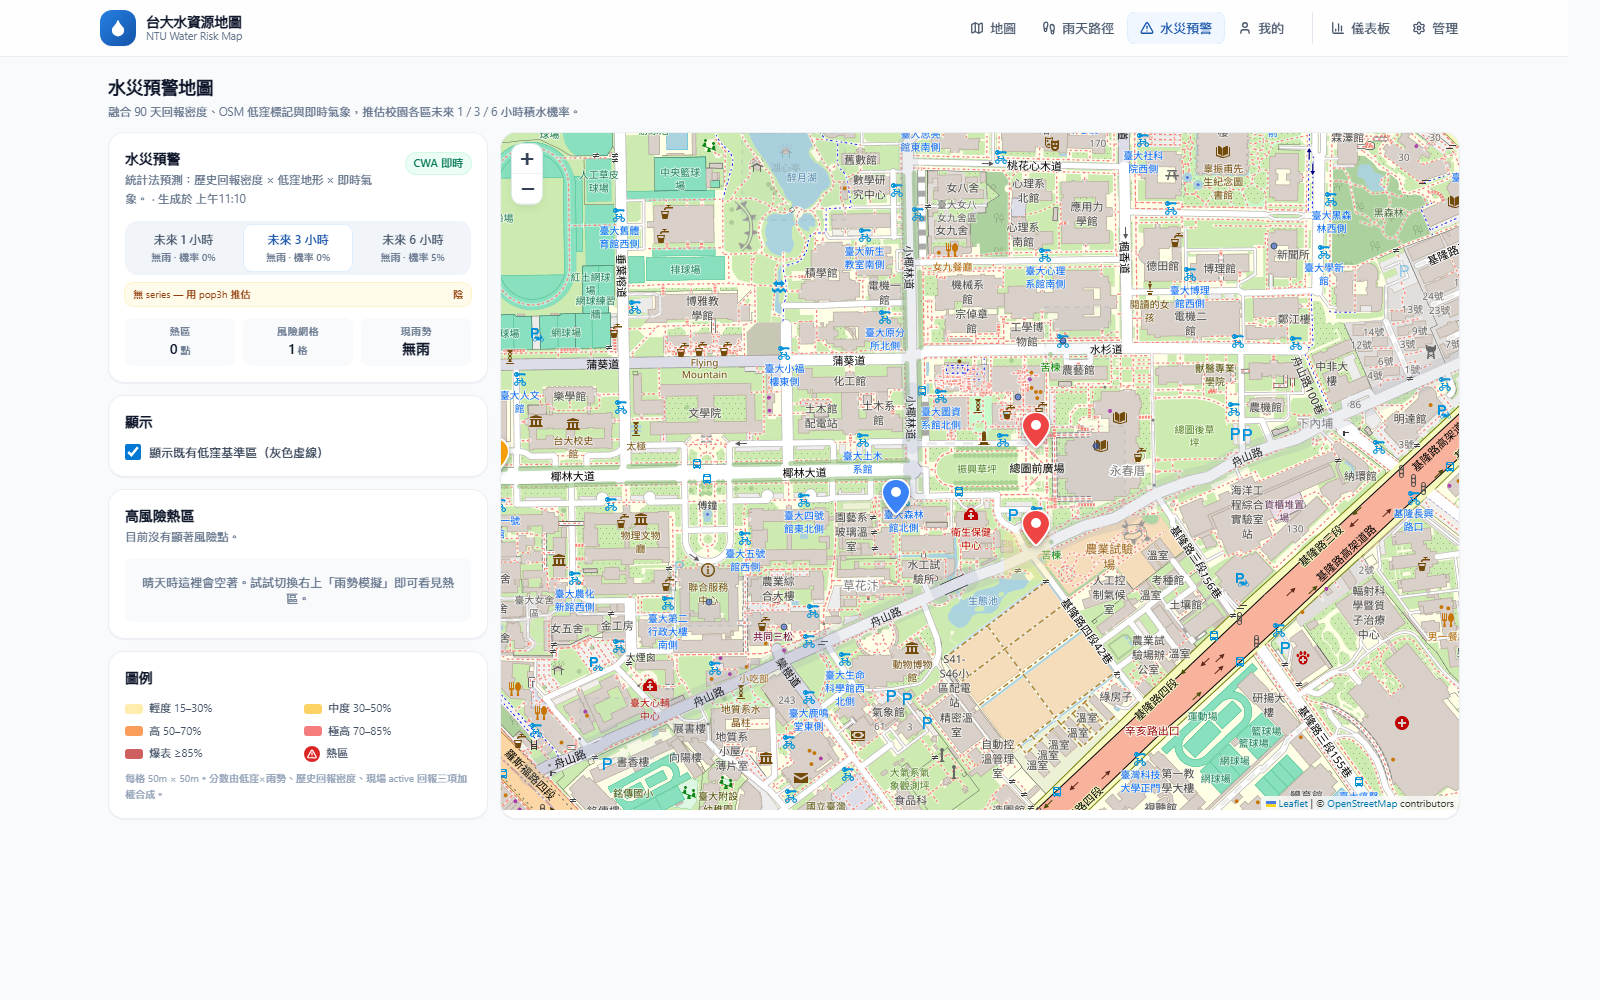
\includegraphics[width=0.96\linewidth]{screens/forecast.png}
\caption{水災預警地圖：圖中所示為「不必擔心」狀態（雨勢小，仍標出 2 個基線熱點）；雨大時格網會自動加密與升溫。}
\end{figure}

預測模型不依賴黑盒 ML，而是\textbf{可解釋的特徵組合}：

\begin{itemize}
\item \textbf{歷史頻率}：將 90 天內的回報投影到 $\approx 20$ m 格網，計算密度；同一格 5 筆遠重於 1 筆。
\item \textbf{地形低窪}：由 \texttt{floodAreas.ts} 中手動標記的 5 個多邊形（小椰林道、醉月湖、總圖前廣場、舟山路低處、校門口）給予加成。
\item \textbf{即時雨勢}：CWA 雨量乘上時間衰減（1\,h vs 6\,h 預測，越遠權重越低）。
\end{itemize}

\clearpage

\subsection{校園水資源儀表板 \texttt{/dashboard}}

儀表板\textbf{不是 markers 的條形圖版}，而是設計給「\emph{校方總務處決策者}」看的：\textbf{解決率}、\textbf{平均處理天數}、\textbf{WoW 變化}（本週 vs 上週）、\textbf{飲水機 SLA}（故障件 / 待換濾心件） —— 都是直接對應 KPI 的指標。資料完全由 \texttt{/api/stats} 即時聚合，零快取，方便 demo 時 console 改 mock 立即生效。

\begin{figure}[H]\centering
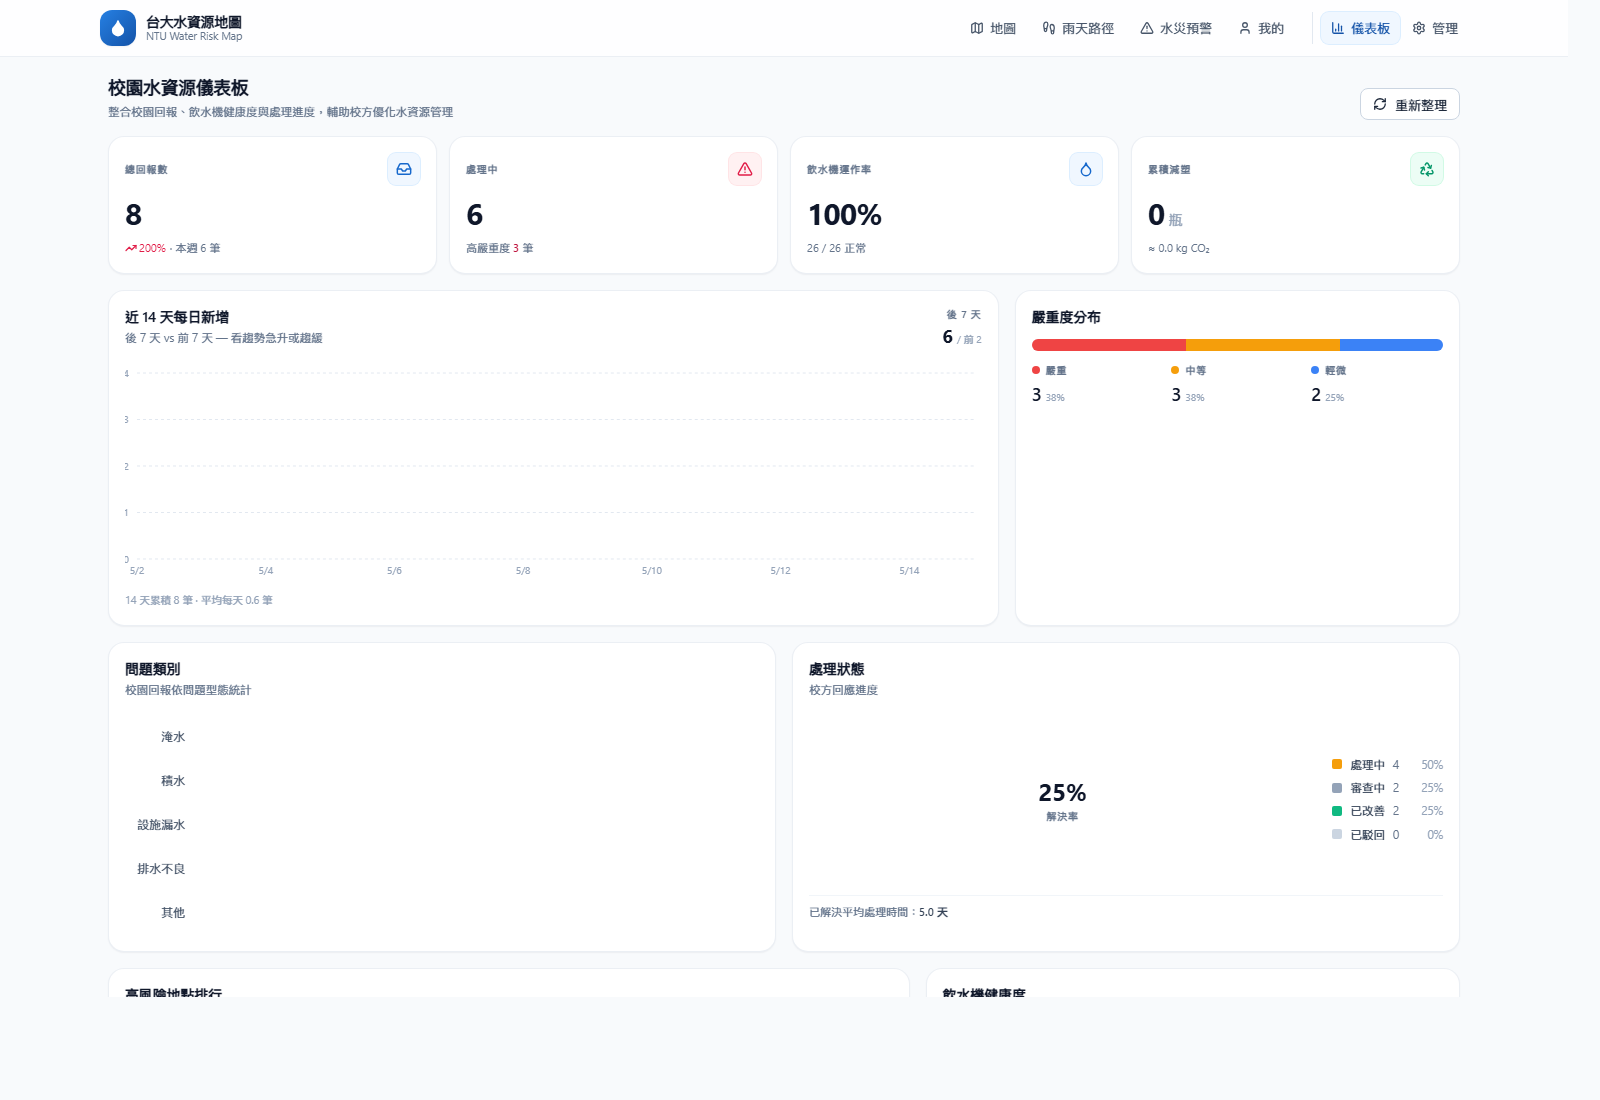
\includegraphics[width=0.96\linewidth]{screens/dashboard.png}
\caption{儀表板上半部：4 張 KPI 卡（總回報、處理中、飲水機健康率、寶特瓶減塑）、14 天每日新增、嚴重度分布、類別／處理狀態。下方還有高風險排行與飲水機健康度。}
\end{figure}

\begin{infobox}
\textbf{\color{brandDeep}儀表板核心 KPI（給校方決策層看）}
\begin{itemize}
\item \textbf{總回報數} 與 \textbf{WoW 變化}：本週相比上週是急升還是趨緩？$\uparrow 200\,\%$ 直接觸發人力盤點。
\item \textbf{處理中件數} 與 \textbf{高嚴重度子集}：判斷積壓量；嚴重件需獨立處理流程。
\item \textbf{飲水機運作率}（健康件 / 總件）+ \textbf{累積減塑寶特瓶}：定期向永續長報告的 ESG 指標。
\item \textbf{14 天日新增趨勢線}：早期辨識梅雨季 onset。
\end{itemize}
\end{infobox}

\clearpage

\subsection{個人成績單 \texttt{/me} — 把回報遊戲化}

設計動機：\textbf{回報意願是專案存活的關鍵}。我們把抽象的「\emph{做好事}」轉化為立即可見的回饋 —— 連續打卡天數（Streak）、行動分數（4 維加權）、徽章解鎖、社群分享文。
14 枚徽章橫跨「\textbf{連續打卡}」「\textbf{飲水機 / 減塑}」「\textbf{通勤路線}」「\textbf{校園回報}」四個行為類別，從新手「\emph{初次入坑}」到極限「\emph{一年水文皇帝}」（連續打卡 365 天），涵蓋短期與長期動機。

\begin{figure}[H]\centering
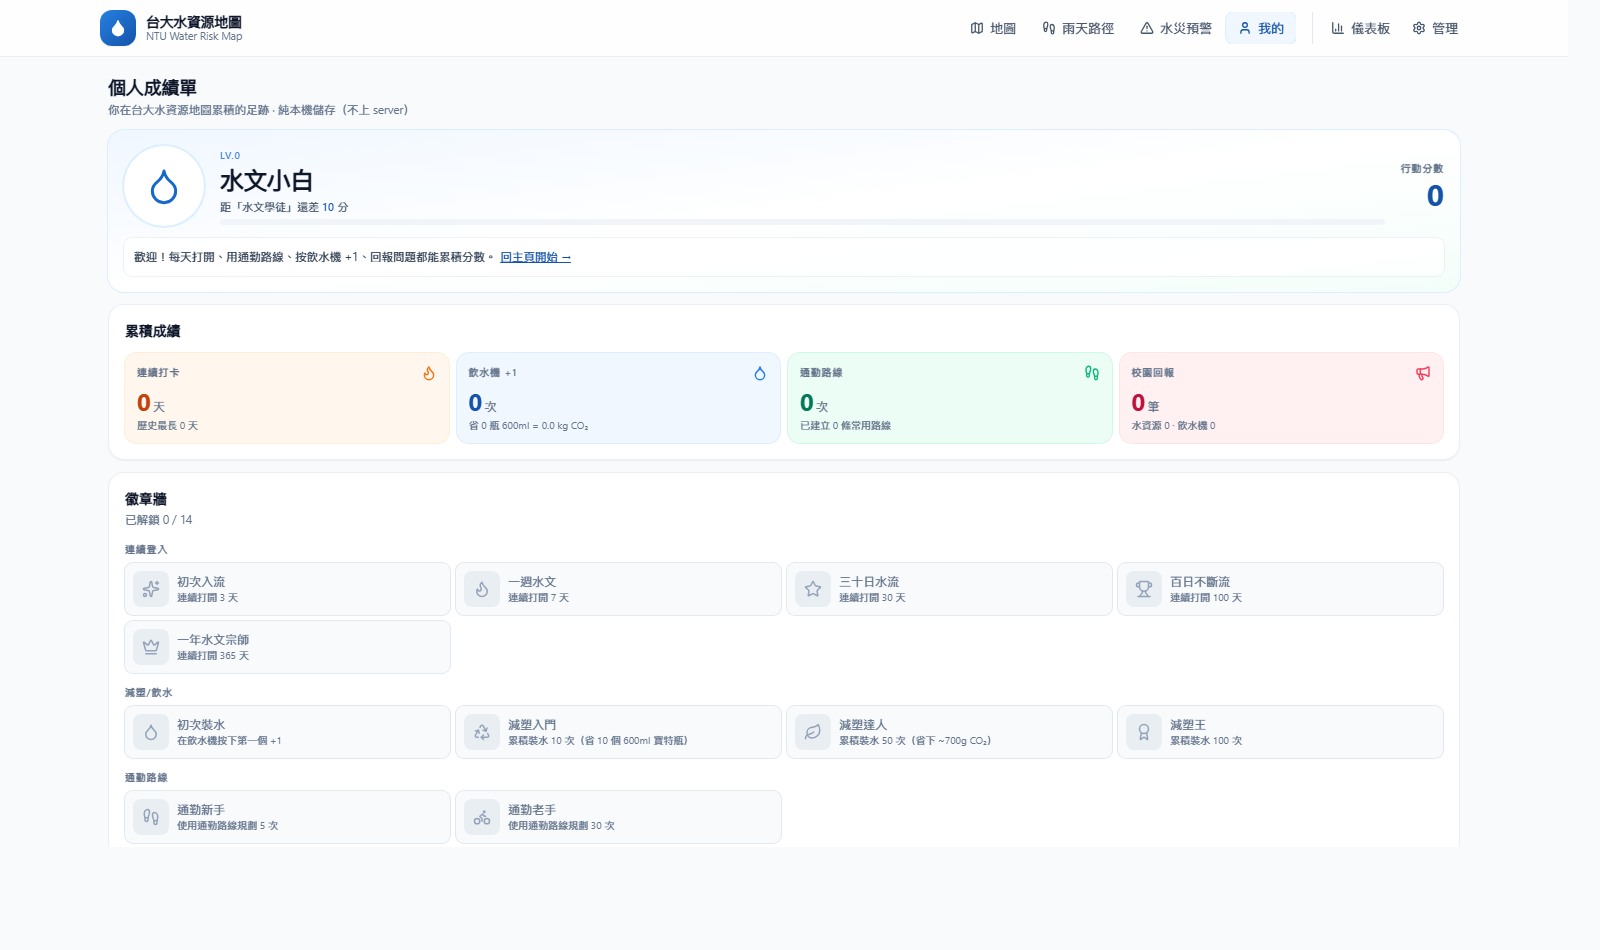
\includegraphics[width=0.96\linewidth]{screens/me.png}
\caption{個人成績單畫面：段位（水文學徒 → 水文大師）、4 格累積成績（連續打卡、飲水機+1、通勤路線、校園回報）、14 枚徽章牆（4 大類別）。所有資料純本機儲存（LocalStorage），零追蹤。}
\end{figure}

\begin{infobox}
\textbf{\color{brandDeep}行動分數設計}
\begin{itemize}
\item \textbf{連續打卡 (Streak)}：每天首次打開地圖即 +1；中斷重置。激勵「每天看一眼」。
\item \textbf{飲水機 +1}：每按一次「我用它裝水了」，行動分數 +2，並累計減塑寶特瓶 / CO\textsubscript{2}\,e。
\item \textbf{通勤路線使用}：使用 \texttt{/route} 規劃並實際走過 +1。
\item \textbf{校園回報}：每筆水資源 / 飲水機回報 +5；管理員確認後再 +5。
\end{itemize}
\end{infobox}

\clearpage

% ═══════════════════════════════════════════════════════
% 5. 演算法細節
% ═══════════════════════════════════════════════════════
\section{演算法細節}

\subsection{校園路網建構：從 OSM 到 Dijkstra-Ready Graph}

最大的工程挑戰是\textbf{真實校園路網}從哪裡來。校內的 22 個地標可以手寫，但「校門口走到綜合體育館」要經過哪些 OSM \texttt{highway=footway} 才不會穿牆？解法是用 \texttt{scripts/build-dense-graph.mjs} 透過 Overpass API 抓取台大校園 bounding box 內所有 \texttt{highway} tagged ways。

\begin{techbox}
\textbf{雙層 GeoJSON 設計}
\begin{itemize}
\item \texttt{src/data/campus.geojson}：22 個\textbf{有名稱的地標}（校門口、傅鐘、共教、活大 \ldots）—— 給 UI start/end 下拉選單用。
\item \texttt{src/data/campus-paths.geojson}：6{,}133 個路徑節點、7{,}248 條邊的\textbf{密集路網}（$\approx$ 3 MB），僅在 server-side 載入。
\end{itemize}

\textbf{邊權標註規則}（從 OSM tags 推論）
\begin{itemize}
\item \texttt{indoor=yes} / \texttt{tunnel=yes} / \texttt{covered=yes} / \texttt{highway=corridor} $\to$ \texttt{covered} $\approx 0.95$
\item \texttt{arcade=yes} $\to$ \texttt{covered} $\approx 0.85$（騎樓）
\item 手動 override 區：椰林大道兩側、行政大樓迴廊、活大周邊
\item 易積水區（\texttt{lowLying}）：小椰林道、醉月湖、總圖前廣場、舟山路低處
\end{itemize}
\end{techbox}

\subsection{加權 Dijkstra 與動態回報整合}

\textbf{Dijkstra 實作}：使用二元堆 priority queue 的 $O((V+E)\log V)$ 標準版本，但在 cost function 中即時讀取「目前 active 的 \texttt{flooding} / \texttt{standing\_water} 回報」並施加懲罰。\textbf{亦即：使用者剛在地圖回報的積水，下一個雨天規劃路徑的同學就會自動繞開。}

效益：在中度雨勢（$r=0.6$）下，\emph{防雨建議路徑}相較\emph{最短路徑}可達遮蔽率提升 $\sim$30\,\%，但只多走 $\sim$50 m。$r$ 為 0 時兩者重疊（不下雨就不繞）。

\subsection{Risk Score 與儀表板聚合}

風險分組與分數計算邏輯：
\[
\mathrm{risk\_score} = \mathrm{report\_count} \times 2 + \mathrm{high\_severity\_count} \times 3 + \mathrm{recent\_7d\_count} \times 2
\]

分數 $\geq 9$ 標記為\textcolor{danger}{\textbf{高風險}}、$\geq 4$ 為\textcolor{warn}{\textbf{中風險}}、其餘為低風險。
這套規則直覺、無需 ML、可解釋 —— 校方看數據時可立即理解「為什麼這個地點上榜」。

\clearpage

% ═══════════════════════════════════════════════════════
% 6. 資料來源
% ═══════════════════════════════════════════════════════
\section{資料來源整合}

本平台整合\textbf{三項外部公開資料}與\textbf{兩項內部資料}：

\begin{table}[H]
\centering
\small
\renewcommand{\arraystretch}{1.4}
\begin{tabular}{@{}p{3.2cm}p{3.2cm}p{10cm}@{}}
\toprule
\textbf{資料源} & \textbf{類型} & \textbf{用途與處理}\\
\midrule
OpenStreetMap & 地理路網（Overpass） & 抓取台大校內所有 \texttt{highway=footway/path/service}，產生 6{,}133 節點路網；用 \texttt{indoor/tunnel/arcade} 推論遮蔽率。\\
中央氣象署 OpenData & 即時氣象 & 觀測 \texttt{O-A0003-001} + 預報 \texttt{F-D0047-061}，抓取大安區雨量、降雨機率、氣溫、濕度。無 \texttt{CWA\_API\_KEY} 時 fallback 至 mock。\\
北水處 OpenData & 飲水機水質 & 與 OSM \texttt{amenity=drinking\_water} 點位融合（\texttt{source: osm / official / merged}），含水質採樣時間與官方狀態。\\
\midrule
內建 Mock Store & In-memory & demo 模式預設啟用，無 Supabase 也可完整跑通；冷啟動會 reset。\\
LocalStorage（client） & 個人成績 & 連續打卡、行動分數、徽章狀態純本機，零追蹤。\\
\bottomrule
\end{tabular}
\caption{資料源整合一覽。所有外部 API 都由 server-side 代理（\texttt{/api/weather}、\texttt{/api/water-stations}），API key 不暴露在 client。}
\end{table}

\subsection{部署與工程實踐}

\begin{accentbox}
\textbf{\color{accent!50!black}工程亮點}
\begin{itemize}
\item \textbf{10 個 API Routes 全 Node runtime}：明確排除 GitHub Pages 等純靜態託管的可能性；選 Vercel hnd1 取得最低台日 RTT。
\item \textbf{重資料 Server-Only}：3 MB 校園路網檔絕不送 client；使用 \texttt{dynamic(\{ssr:false\})} 處理 Leaflet 的 \texttt{window} 依賴。
\item \texttt{maxDuration:30s}：\texttt{/api/route} 與 \texttt{/api/forecast} 設置長 timeout 容納 Dijkstra 與 90 天熱力預測。
\item \textbf{Mock / Real 雙模式}：環境變數一鍵切換，期末展示時零配置上線。
\item \textbf{Error Boundaries}：頁面級 \texttt{error.tsx} + 全域 \texttt{global-error.tsx} 雙層保護，避免地圖載入失敗整站白屏。
\end{itemize}
\end{accentbox}

\vspace{0.3em}\noindent\textbf{\large\color{ink}6.2\quad API 端點清單}
\vspace{0.5em}

{\small
\renewcommand{\arraystretch}{1.1}
\begin{tabular}{@{}p{5.4cm}l p{7.4cm}@{}}
\toprule
\textbf{Endpoint} & \textbf{Method} & \textbf{用途}\\
\midrule
\texttt{/api/reports} & GET\,/\,POST & 取得 / 新增水資源回報（含圖片上傳）\\
\texttt{/api/reports/[id]} & PATCH\,/\,DELETE & 管理端修改狀態 / 加管理員 note / 刪除\\
\texttt{/api/reports/[id]/confirm} & POST & 眾包確認（\texttt{still\_exists} / \texttt{resolved}）\\
\texttt{/api/stats} & GET & 儀表板聚合（KPI + 趨勢 + 排行 + 飲水機 SLA）\\
\texttt{/api/weather} & GET & CWA OpenData 代理，金鑰 server-side 保護\\
\texttt{/api/route} & POST & 雨天 Dijkstra；起終點 + mode + avoidWater\\
\texttt{/api/forecast} & GET & 1 / 3 / 6 小時積水機率格網\\
\texttt{/api/water-stations} & GET & 飲水機點位（OSM + 北水處融合）\\
\texttt{/api/water-stations/[id]/report} & POST & 飲水機回報（broken / fixed / refill）\\
\texttt{/api/path-geometry} & POST & 路徑幾何輔助（snap to road）\\
\bottomrule
\end{tabular}
}

% ═══════════════════════════════════════════════════════
% 7. 設計 + 結論 + 參考（讓 LaTeX 自動接續，避免無謂空頁）
% ═══════════════════════════════════════════════════════
\section{視覺設計系統}

整套 UI 採用「\textbf{Apple 等級的克制 + 顏色語意化}」原則：

\begin{itemize}
\item \textbf{品牌色 \texttt{\#0EA5E9}（Sky 500）}：呼應水的清澈，主 CTA、活躍連結、品牌徽。
\item \textbf{嚴重度色階}：\textcolor{danger}{$\bullet$} 紅 = 嚴重、\textcolor{warn}{$\bullet$} 橙 = 中等、\textcolor{brand}{$\bullet$} 藍 = 輕微 —— 與地圖 marker、儀表板 chart、表格 badge 共用，全站視覺語意一致。
\item \textbf{icon library}：全站 lucide-react 線性圖示，零 emoji，避免跨平台 fallback 差異。
\item \textbf{字級系統}：標題 11--16 px、內文 12.5--13 px、KPI 數字 30+ px tabular-nums 對齊。
\item \textbf{動效}：\texttt{animate-fade-in} + \texttt{ease-soft-out} 自訂 curve，整站轉場 250 ms，乾淨不浮誇。
\end{itemize}

\section{結論與未來工作}

本專題完成了一套\textbf{可上線、可擴充、有實證價值}的校園水資源 web app，
不只是課堂作業 demo，而是已部署於 Vercel、有 6 個頁面、10 個 API、整合 3 個外部資料源的\emph{產品級實作}。
我們把「水資源管理」這個傳統工程議題，重新詮釋為「\emph{資料 + 介面 + 行為}」的三層問題，
並用最務實的技術組合 —— Next.js + Leaflet + OSM + Dijkstra —— 做出可立即使用的工具。

\subsection{未來工作}

\begin{enumerate}
\item \textbf{接入 NTU SSO 或 Magic Link}：取代目前的密碼登入，提升管理端安全性。
\item \textbf{推播通知}：當使用者通勤路線上出現新積水回報，主動推送 Web Push。
\item \textbf{歷史趨勢回放}：把 90 天熱力預測加上 timeline scrubber，可回看 1 個月前的某天校園水情。
\item \textbf{ML 路徑預測}：當回報數 $> 1{,}000$ 時，可嘗試以 LightGBM 取代手動係數，預測「未來 1 小時哪段路會出現新積水」。
\item \textbf{校方 API 對接}：與台大總務處事務組系統 API 串接，已解決的回報自動同步。
\end{enumerate}

\clearpage
\renewcommand{\refname}{\color{brandDeep}\Large\bfseries 參考文獻\quad References\vspace{-0.2em}\\\color{brand}\rule{\linewidth}{0.6pt}}
\addcontentsline{toc}{section}{References}

\begin{thebibliography}{99}
\small\setlength{\itemsep}{3pt}

\bibitem{nextjs} Vercel Inc. (2024). \emph{Next.js 14 — The React Framework for the Web}.\\
\url{https://nextjs.org/docs}

\bibitem{leaflet} Agafonkin, V. (2024). \emph{Leaflet — An Open-Source JavaScript Library for Mobile-Friendly Interactive Maps}.\\
\url{https://leafletjs.com/}

\bibitem{osm} OpenStreetMap Foundation. (2024). \emph{OpenStreetMap Wiki — Map Features and Overpass API Documentation}.\\
\url{https://wiki.openstreetmap.org/}

\bibitem{cwa} 交通部中央氣象署 (2024). \emph{氣象資料開放平臺 —— 觀測 O-A0003-001 \& 預報 F-D0047-061}.\\
\url{https://opendata.cwa.gov.tw/}

\bibitem{twd} 臺北自來水事業處 (2024). \emph{飲水機水質開放資料 OpenData}.\\
\url{https://data.water.gov.taipei/}

\bibitem{dijkstra} Dijkstra, E. W. (1959). A note on two problems in connexion with graphs. \emph{Numerische Mathematik}, 1(1), 269--271.

\bibitem{recharts} Recharts Group. (2024). \emph{Recharts — A composable charting library built on React components}.\\
\url{https://recharts.org/}

\bibitem{supabase} Supabase Inc. (2024). \emph{Supabase — The Open Source Firebase Alternative}.\\
\url{https://supabase.com/docs}

\bibitem{tailwind} Tailwind Labs Inc. (2024). \emph{Tailwind CSS — Utility-first CSS framework}.\\
\url{https://tailwindcss.com/}

\bibitem{vercel} Vercel Inc. (2024). \emph{Vercel Platform — Deploy Next.js Apps}.\\
\url{https://vercel.com/docs}

\bibitem{lucide} Lucide Contributors. (2024). \emph{Lucide — Beautiful \& consistent icon toolkit made by the community}.\\
\url{https://lucide.dev/}

\end{thebibliography}

\end{document}
